%%%%%%%%%%%%%%%%%%%%%%%%%%%%%%%%%%%%%%%%%%%%%%%%%%%%%%%%%%%%%%%%%%%%%%%%%%%%%%%%%%%%%%%%%%%%%%%%%%%%
% Project Requirements Specification Report
% Authors: Michael Galliers and James Miller
% Course: CSC 440
%%%%%%%%%%%%%%%%%%%%%%%%%%%%%%%%%%%%%%%%%%%%%%%%%%%%%%%%%%%%%%%%%%%%%%%%%%%%%%%%%%%%%%%%%%%%%%%%%%%%

\documentclass[12pt]{article}
\usepackage[utf8]{inputenc}
\usepackage{graphicx}
\usepackage{float}
\usepackage{tocloft}
% Page margins
\usepackage[letterpaper, portrait, margin=1in]{geometry}

% Document configuration

% Section numbering
\renewcommand \thesection{\Roman{section}}
\renewcommand \thesubsection{\Alph{subsection}.}

% Environment config for requirements
%  - Configures formatting of the section heading and numbered, nested lists
\newenvironment{requirement}[1]
{
    % Format requirement sections (R1. ...)
    \renewcommand{\thesubsubsection}{R\arabic{subsubsection}.}
    % Format nested, numbered lists (1.1, 1.1.1, 1.1.1.1, ...)
    \renewcommand{\labelenumi}{
        \arabic{subsubsection}.\arabic{enumi}
    }
    \renewcommand{\labelenumii}{
        \arabic{subsubsection}.\arabic{enumi}.\arabic{enumii}
    }
    \renewcommand{\labelenumiii}{
        \arabic{subsubsection}.\arabic{enumi}.\arabic{enumii}.\arabic{enumiii}
    }
    \renewcommand{\labelenumiv}{
        \arabic{subsubsection}.\arabic{enumi}.\arabic{enumii}.\arabic{enumiii}.\arabic{enumiv}
    }
    % Create the subsubsection for the requirement
    \subsubsection{#1}
    \begin{enumerate}
}
{
    \end{enumerate}
}

\newcommand{\dictitem}[1]{\item \textbf{#1}:}
% Data dictionary environment
\newenvironment{dict}
{
    \begin{itemize}
}
{
    \end{itemize}
}

% Set path to all graphics
\graphicspath{{figures/}{build/diagrams/}}

% Do paragraph indenting after section tags
\usepackage{indentfirst}

% Adjust space between numbers and headings in table of contents
\addtolength{\cftsecnumwidth}{12pt}
\addtolength{\cftsubsubsecnumwidth}{-10pt}


\author{Michael Galliers and James Miller}
\title{CSC 440 - Requirements Specification Report}


\begin{document}

\begin{titlepage}
\maketitle
\end{titlepage}

\newpage
    \tableofcontents
\newpage

% No styling
\thispagestyle{empty}
% Include a table of figures
\listoffigures
% New page
\newpage

\section{Introduction}
\subsection{Problem Statement}
As EKU college students, we the authors have firsthand experience with the difficulties of
grade/progress management. The tools already used by the college for grade management have their
flaws. Many professors either do not setup the grading categories and weights properly, or they
choose to not use BlackBoard for tracking grades at all. Also, BlackBoard does not have the ability
to give advanced insights for student grades other than simple weighted averages or totals.

Students can choose to manage their grades on their own, either using technology, such as
spreadsheets, or pen and paper. Students who do this are able to gain more insights into their
progress in courses, but it can be very time consuming to setup spreadsheets or do computations by
hand, especially when predicting grades needed on an assignment.

\subsection{Proposal}
As a solution to these problems, we propose a software system for grade and progress tracking. The
system shall have 2 main related components: one for grade tracking and one for major/concentration
progress tracking. The grade tracking system will allow students to easily enter and track their
grades across colleges, semesters, courses, and categories (homework, exams, etc.). Various views on
the user interface will display grades/scores using visual elements and animations, making it easy
for students to see how well they are doing.

The second component of the application is a progress tracker for majors and concentrations.
Information provided through the grade tracking feature, coupled with course requirements structures
will allow students to view their progress across multiple majors and concentrations.

\section{System Description}
The system shall have a user account management component to keep track of students, including the
ability to register, login, edit account, and logout. When a student logs into the system, the
student shall see a dashboard containing the most relevant information and navigation links. From
there, the student will also be able to access the system menu, allowing them to navigate to either
the grade tracking component or the progress tracking component.

\subsection{Grade Tracking Component}
\noindent
The grade tracking component shall have views for the following items:

\begin{enumerate}
    \item All semesters (root grade tracking view)
    \item Courses in a semester
    \item Details of a course (including categories and grade entries)
\end{enumerate}

The \textit{All Semesters} view shall allow the student to navigate to a particular semester,
add/remove a semester in which they are enrolled, and view statistics about his/her grades in that
semester.

The \textit{Courses} view shall display the courses that are in a particular semester. The student
shall be able to add/remove/edit courses, view statistics for grades in each course, and navigate
to any of the courses.

The \textit{Course Detail} view shall display all remaining details for a particular course. This
includes the statistics of a student's grades in the course, the grading categories of the course,
and the grade entries themselves. The student shall also have the ability to add/remove/edit
categories and grade entries.

\subsection{Progress Tracking Component}
\noindent
The progress tracking component shall allow students to track their progress across major
concentrations. This component shall have the following hierarchical views:

\begin{enumerate}
    \item Colleges (root progress tracking view)
    \item Majors
    \item Concentrations
    \item Concentration progress
\end{enumerate}

The \textit{Colleges} view shall display the colleges in which the student is enrolled and allow
him/her to navigate to the \textit{Majors} view for that college. The student shall also have the
ability to add/remove colleges which he/she is enrolled in.

The \textit{Majors} view shall display the majors of the college which was navigated from that the
student is enrolled in. The student shall be able to add/remove majors which he/she is enrolled in
and also navigate to the \textit{Concentrations} view for a particular major.

The \textit{Concentrations} view shall display \textbf{all} the concentrations of the major which
was navigated from, broken up into 2 sections: one for the concentration(s) the student in enrolled
in and one for all other concentrations. The student shall be able to add/remove concentrations
which they are enrolled in and navigate to the \textit{Concentration progress} view.

The \textit{Concentration progress} view shall display visuals for the student's progress in the
concentration, including overall progress and individual courses completed. This view shall be based
on courses the student has entered through the grade tracking component.

\section{System Requirements}
\subsection{Functional Requirements}

% Some common text/sequences that are used a lot...
\newcommand{\sysshall}{The system shall }
\newcommand{\stushall}{The student shall }
\newcommand{\usershall}{The user shall }
\newcommand{\loginpage}{\sysshall display the login page.}
\newcommand{\mainmenu}{\sysshall display the main menu.}
\newcommand{\clickmainmenu}{\stushall click the \textbf{Main Menu} button}
\newcommand{\redirecthome}{\sysshall redirect the student to the homepage.}
\newcommand{\gotohome}{
    \item \clickmainmenu
    \item \mainmenu
}

\begin{requirement}{\sysshall allow a user to register for an account}
    \item \loginpage
    \item \usershall click the \textbf{Register} button.
    \item \sysshall display the \emph{Registration} page.
    \item \usershall enter the requested information.
    \item \usershall click the \textbf{Register} button.
    \item \sysshall validate the information entered by the user.
    \begin{enumerate}
        \item If the entered information is invalid, the system shall display warnings next to the
        relevant fields.
    \end{enumerate}
    \item \redirecthome
\end{requirement}

\begin{requirement}{\sysshall allow a student to login to his/her account}
    \item \loginpage
    \item \stushall enter his/her login credentials.
    \item \sysshall validate the credentials.
    \begin{enumerate}
        \item If the credentials are not valid, the system shall display warnings next to the
        fields with errors.
    \end{enumerate}
    \item \redirecthome
\end{requirement}

\begin{requirement}{\sysshall allow a student to logout of his/her account}
    \item \mainmenu
    \item \stushall click the \textbf{Logout} button.
    \item \loginpage
\end{requirement}

\begin{requirement}{\sysshall allow a student to view progress in a concentration}
    \item \mainmenu
    \item \stushall click the \textbf{Concentration Progress} button.
    \item \sysshall display the \emph{Concentration Progress} page.
    \item \stushall select the college which the concentration is in.
    \item \stushall select the major which the concentration is in.
    \item \stushall select the concentration.
    \item \stushall click the \textbf{Load Progress} button.
    \item \sysshall display the concentration requirement structure.
    \gotohome
\end{requirement}

% Shortcut for navigating to semester page
\newcommand{\navsemesters}{
    \item \mainmenu
    \item \stushall click the \textbf{Semesters} button.
    \item \sysshall display the semesters the student is enrolled in.
}

\begin{requirement}{\sysshall allow a student to view enrolled semesters}
    \navsemesters
    \gotohome
\end{requirement}

\begin{requirement}{\sysshall allow a student to add/remove enrolled semesters}
    \navsemesters
    \item \stushall click the \textbf{Add Semester} button.
    \item \sysshall display the \emph{Add Semester} form.
    \item \stushall select the semester to add.
    \item \stushall click the \textbf{Save} button.
    \item \sysshall add that semester to the semesters shown.
    \item \stushall click the \textbf{Delete} button next to one of the semesters.
    \item \sysshall display a delete confirmation message.
    \item \stushall click the \textbf{Yes, Delete} button.
    \item \sysshall remove that semester from the semesters shown.
    \gotohome
\end{requirement}

% Shortcut for navigating to enrolled courses
\newcommand{\navcourses}{
    \navsemesters
    \item \stushall click the chosen semester.
    \item \sysshall display the courses the student is enrolled in, in the selected semester.
}

\begin{requirement}{\sysshall allow a student to view enrolled courses}
    \navcourses
    \gotohome
\end{requirement}

\begin{requirement}{\sysshall allow a student to add/remove enrolled courses}
    \navcourses
    \item \stushall click the \textbf{Add Course} button.
    \item \sysshall display the \emph{Add Course} form.
    \item \stushall select the course to add.
    \item \stushall click the \textbf{Save} button.
    \item \sysshall add that course to the courses shown.
    \item \stushall click the \textbf{Delete} button next to one of the courses.
    \item \sysshall display a delete confirmation message.
    \item \stushall click the \textbf{Yes, Delete} button.
    \item \sysshall remove that course from the courses shown.
    \gotohome
\end{requirement}

% Shortcut for navigating to course details
\newcommand{\navcoursedetails}{
    \navcourses
    \item \stushall click the chosen course.
    \item \sysshall display the course details for the selected course.
}

\begin{requirement}{\sysshall allow a student to view course details}
    \navcoursedetails
    \gotohome
\end{requirement}

\begin{requirement}{\sysshall allow a student to add/edit/remove grade entries}
    \navcoursedetails
    \item \stushall click the \textbf{Add Grade Entry} button under one of the categories.
    \item \sysshall display the \emph{Grade Entry} form.
    \item \stushall enter the information required.
    \item \stushall click the \textbf{Save} button.
    \begin{enumerate}
        \item If any of the fields are invalid, the system shall display warnings next to those
        fields which are invalid.
    \end{enumerate}
    \item \sysshall add the new grade entry to the grade entries shown.
    \item \stushall click the \textbf{Edit} button next to one of the grade entries.
    \item \sysshall display the \emph{Grade Entry} form, populated with the selected grade entry's
    information.
    \item \stushall edit the grade entry information.
    \item \stushall click the \textbf{Save} button.
    \begin{enumerate}
        \item If any of the fields are invalid, the system shall display warnings next to those
        fields which are invalid.
    \end{enumerate}
    \item \sysshall update the grade entry information on the course details page accordingly.
    \item \stushall click the \textbf{Edit} button next to one of the courses.
    \item \sysshall display the \emph{Grade Entry} form, populated with the selected grade entry's
    information.
    \item \stushall click the \textbf{Delete} button.
    \item \sysshall display a delete confirmation message.
    \item \stushall click the \textbf{Yes, Delete} button.
    \item \sysshall remove that grade entry from the course details page.
    \gotohome
\end{requirement}

% \subsection{Non-functional Requirements}

% \subsection{Domain Requirements}

\begin{figure}[p!]
  \section{Use-case Diagram}
  \centering
  \includegraphics[width=0.8\linewidth]{use_case_diagram.pdf}
  \caption{Use-case Diagram}
\end{figure}

\clearpage

\begin{figure}[p!]
  \section{Class Diagram}
  \centering
  \includegraphics[width=0.90\linewidth]{class_diagram.pdf}
  \caption{Class Diagram}
\end{figure}

\clearpage

\begin{figure}[p!]
  \section{Sequence Diagrams}
  \subsection{Register Sequence Diagram}
  \centering
  \includegraphics[width=\linewidth]{register_sequence_diagram.pdf}
  \caption{Register Sequence Diagram}
\end{figure}

\begin{figure}[p!]
  \subsection{Login Sequence Diagram}
  \centering
  \includegraphics[width=\linewidth]{login_sequence_diagram.pdf}
  \caption{Login Sequence Diagram}
\end{figure}

\begin{figure}[p!]
  \subsection{Logout Sequence Diagram}
  \centering
  \includegraphics[width=\linewidth]{logout_sequence_diagram.pdf}
  \caption{Logout Sequence Diagram}
\end{figure}

\begin{figure}[p!]
  \subsection{Concentration Progress Sequence Diagram}
  \centering
  \includegraphics[width=\linewidth]{concentration_progress_sequence_diagram.pdf}
  \caption{Concentration Progress Sequence Diagram}
\end{figure}

\begin{figure}[p!]
  \subsection{View Semesters Sequence Diagram}
  \centering
  \includegraphics[width=\linewidth]{view_semesters_sequence_diagram.pdf}
  \caption{View Semesters Sequence Diagram}
\end{figure}

\begin{figure}[p!]
  \subsection{Add/Remove Semesters Sequence Diagram}
  \centering
  \includegraphics[width=\linewidth]{add_remove_semesters_sequence_diagram.pdf}
  \caption{Add/Remove Semesters Sequence Diagram}
\end{figure}

\begin{figure}[p!]
  \subsection{View Courses Sequence Diagram}
  \centering
  \includegraphics[width=\linewidth]{view_courses_sequence_diagram.pdf}
  \caption{View Courses Sequence Diagram}
\end{figure}

\begin{figure}[p!]
  \subsection{Add/Remove Courses Sequence Diagram}
  \centering
  \includegraphics[width=\linewidth]{add_remove_courses_sequence_diagram.pdf}
  \caption{Add/Remove Courses Sequence Diagram}
\end{figure}

\begin{figure}[p!]
  \subsection{View Course Details Sequence Diagram}
  \centering
  \includegraphics[width=\linewidth]{view_course_details_sequence_diagram.pdf}
  \caption{View Course Details Sequence Diagram}
\end{figure}

\begin{figure}[p!]
  \subsection{Add/Edit/Remove Grade Entries Sequence Diagram}
  \centering
  \includegraphics[width=0.55\linewidth]{add_edit_remove_grade_entries_sequence_diagram.pdf}
  \caption{Add/Edit/Remove Grade Entries Sequence Diagram}
\end{figure}

\begin{figure}[p!]
  \section{State Diagram}
  \centering
  \includegraphics[width=\linewidth]{state_diagram.pdf}
  \caption{State Diagram}
\end{figure}

\begin{figure}[p!]
  \section{Activity Diagrams}
  \subsection{Register Activity Diagram}
  \centering
  \includegraphics[width=0.95\linewidth]{register_activity_diagram.pdf}
  \caption{Register Activity Diagram}
\end{figure}

\begin{figure}[p!]
  \subsection{Login Activity Diagram}
  \centering
  \includegraphics[width=0.75\linewidth]{login_activity_diagram.pdf}
  \caption{Login Activity Diagram}
\end{figure}

\begin{figure}[p!]
  \subsection{Logout Activity Diagram}
  \centering
  \includegraphics[width=\linewidth]{logout_activity_diagram.pdf}
  \caption{Logout Activity Diagram}
\end{figure}

\begin{figure}[p!]
  \subsection{Concentration Progress Activity Diagram}
  \centering
  \includegraphics[width=\linewidth]{concentration_progress_activity_diagram.pdf}
  \caption{Concentration Progress Activity Diagram}
\end{figure}

\begin{figure}[p!]
  \subsection{View Semesters Activity Diagram}
  \centering
  \includegraphics[width=\linewidth]{view_semesters_activity_diagram.pdf}
  \caption{View Semesters Activity Diagram}
\end{figure}

\begin{figure}[p!]
  \subsection{Add/Remove Semesters Activity Diagram}
  \centering
  \includegraphics[width=\linewidth]{add_remove_semesters_activity_diagram.pdf}
  \caption{Add/Remove Semesters Activity Diagram}
\end{figure}

\begin{figure}[p!]
  \subsection{View Courses Activity Diagram}
  \centering
  \includegraphics[width=\linewidth]{view_courses_activity_diagram.pdf}
  \caption{View Courses Activity Diagram}
\end{figure}

\begin{figure}[p!]
  \subsection{Add/Remove Courses Activity Diagram}
  \centering
  \includegraphics[width=\linewidth]{add_remove_courses_activity_diagram.pdf}
  \caption{Add/Remove Courses Activity Diagram}
\end{figure}

\begin{figure}[p!]
  \subsection{View Course Details Activity Diagram}
  \centering
  \includegraphics[width=0.75\linewidth]{view_course_details_activity_diagram.pdf}
  \caption{View Course Details Activity Diagram}
\end{figure}

\begin{figure}[p!]
  \subsection{Add/Edit/Remove Grade Entries Activity Diagram}
  \centering
  \includegraphics[width=0.5\linewidth]{add_edit_remove_grade_entries_activity_diagram.pdf}
  \caption{Add/Edit/Remove Grade Entries Activity Diagram}
\end{figure}

\begin{figure}[p!]
  \section{Database Design}
  \subsection{ER Schema}
  \centering
  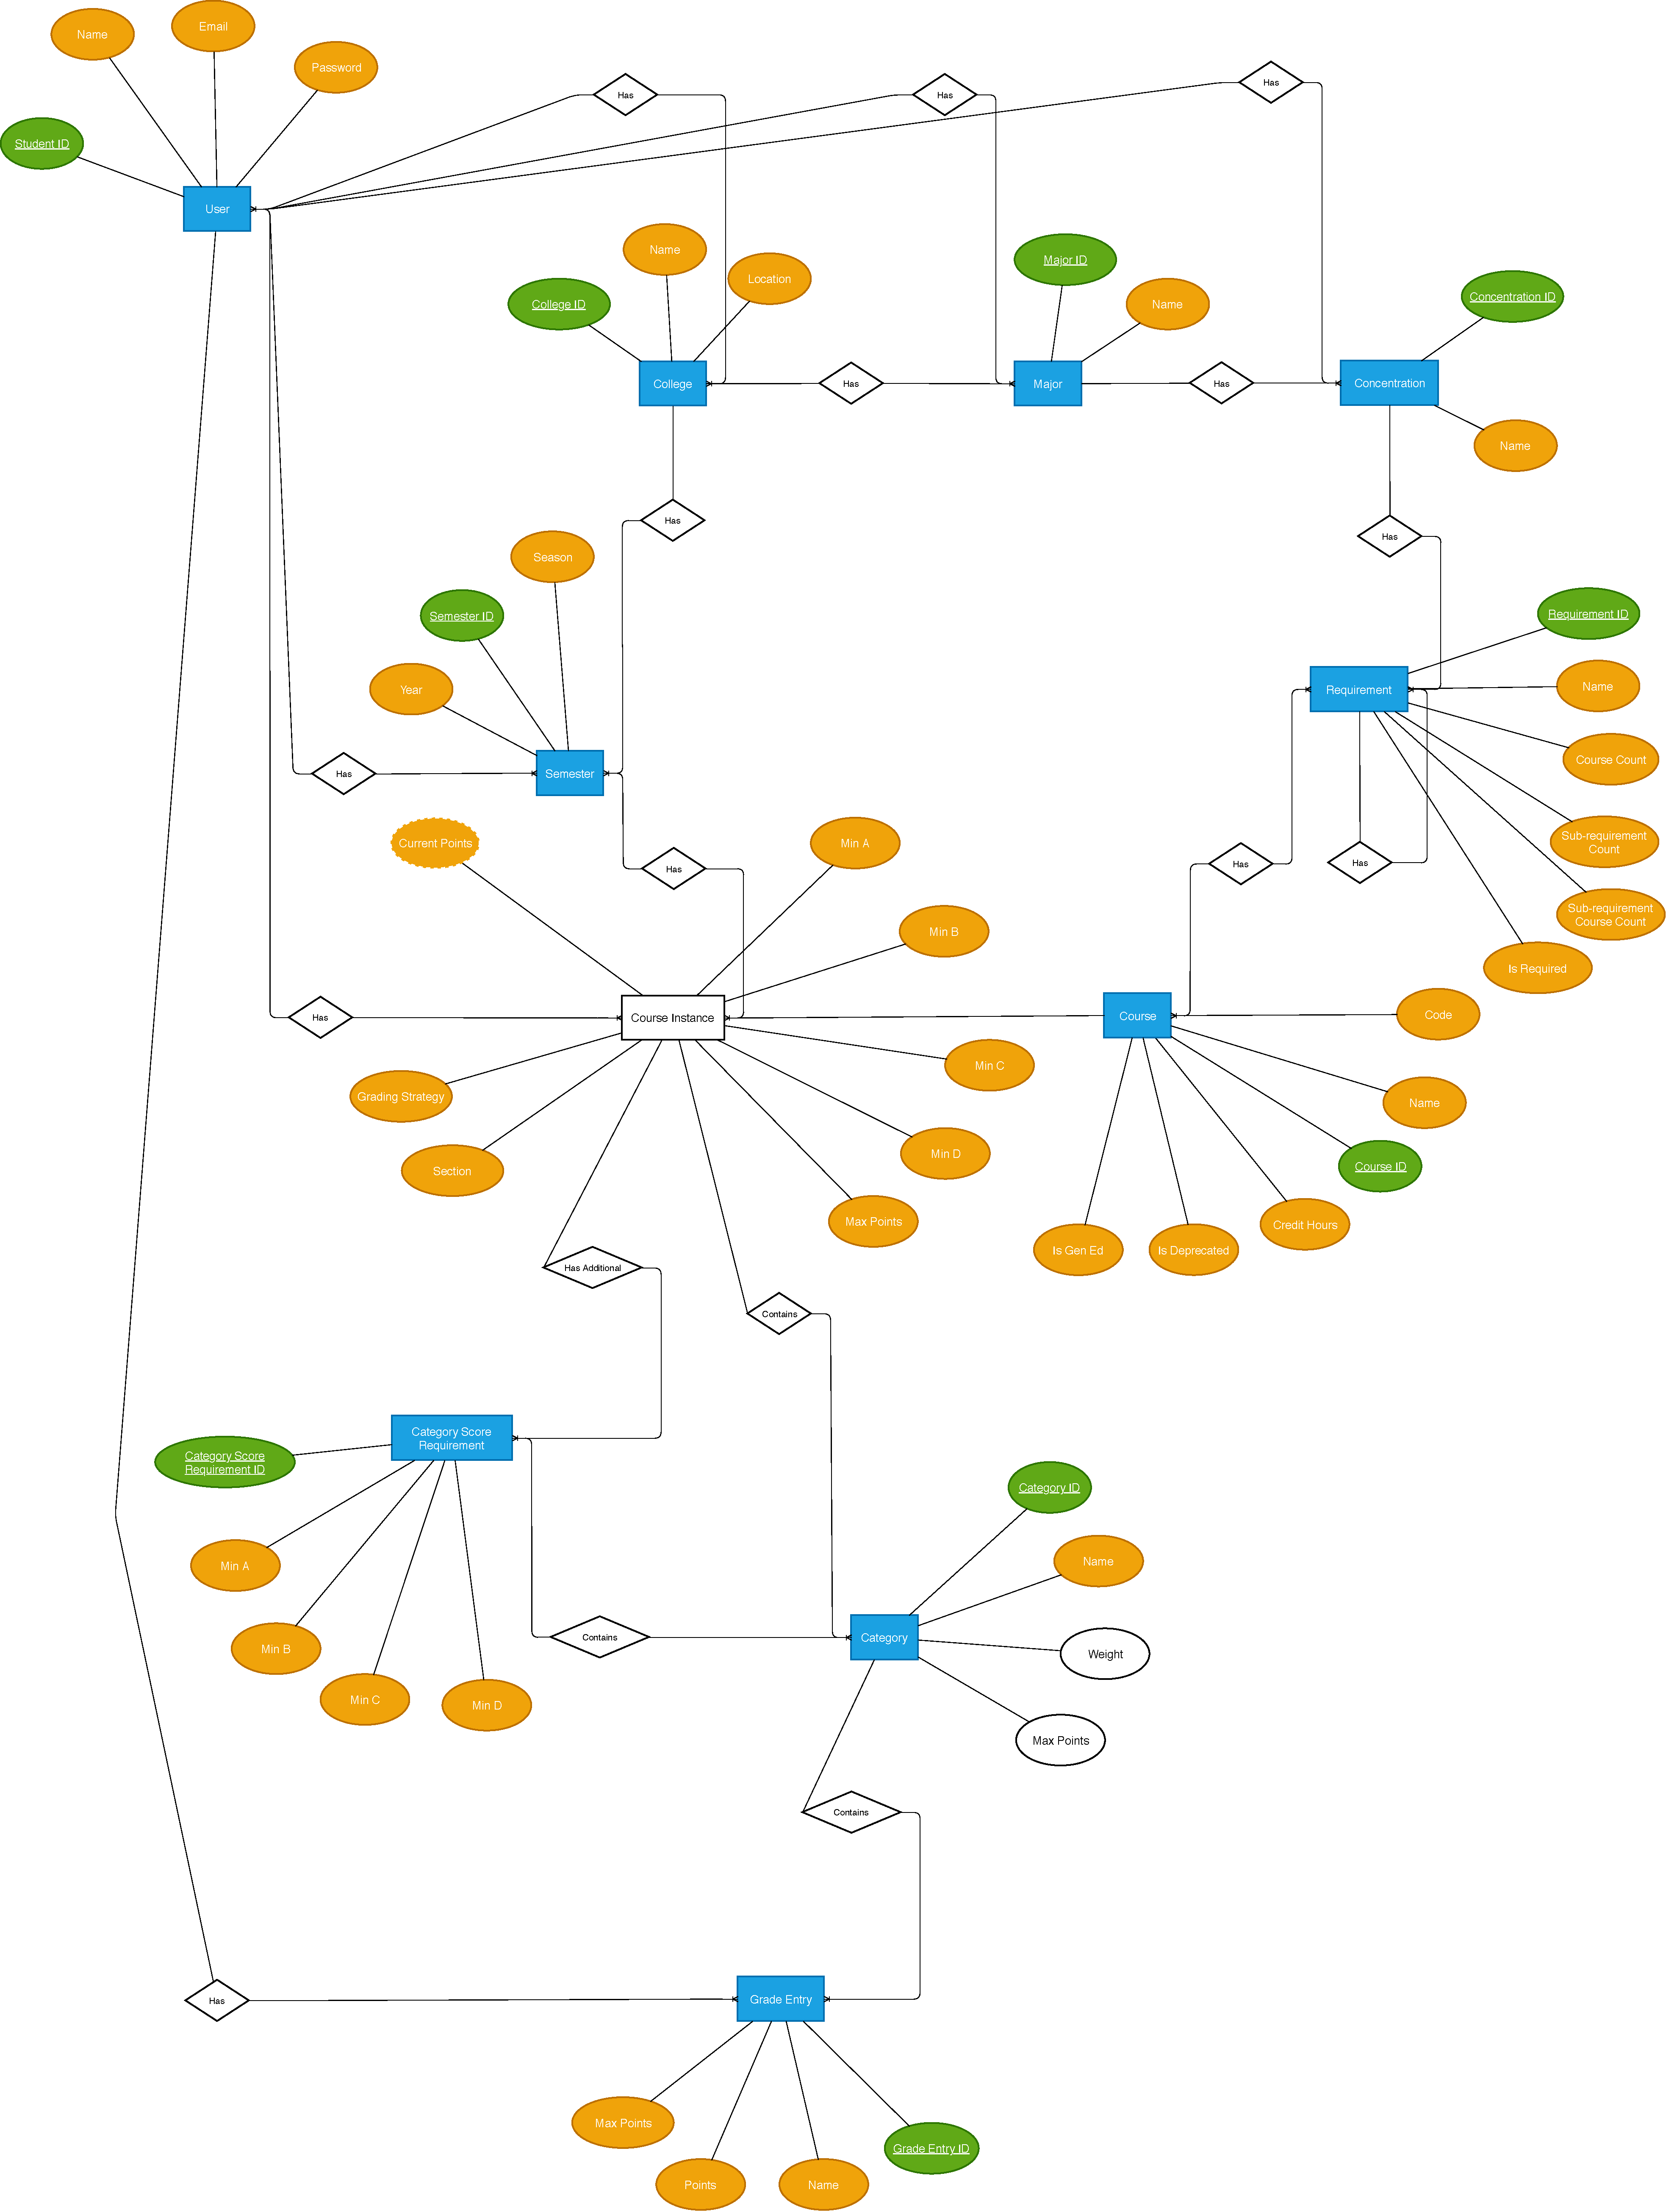
\includegraphics[width=0.90\linewidth]{database_erd.pdf}
  \caption{Database ERD}
\end{figure}

\clearpage

% \subsection{Table Schema}

\section{Conclusion}
As a result of developing this software system, we hope to have a direct effect on other college
student's lives, making it significantly easier for them to monitor and keep track of their grades.
In our role as developers, we intend to use this project to gain further knowledge into how modern
software systems are built and operate. Our goal beyond the immediate scope of this project, is to
make the system as easy as possible to setup and scale, allowing other colleges and educational
organizations to quickly set it up and use it.

\section{Dictionary}
\begin{dict}
    \dictitem{Semester} A single semester of education consisting of courses. Each semester can
    be associated with a different educational institution; consistency is not required.
    \dictitem{Course} Any educational course/class occurring within a particular semester.
    \dictitem{Section} An equally weighted or logically grouped collection of material within a
    particular course (e.g. Homework, Tests, etc.).
    \dictitem{Grade Entry} A graded piece of material associated with a particular section 
    (e.g. Homework 2, Exam 1, etc.).
    \dictitem{User} A new user of the software system who does not yet have an account.
    \dictitem{Student} A user of the software system who has an account and is a college student.
    \dictitem{Requirement Structure} A recursive structure defining the required courses to complete
    a concentration.
\end{dict}

\end{document}
